%-----------------------------------------------------------------------------------------------------
%        روش اجرا.: 2 بار F1 ، 2 بار  F11(به منظور تولید مراجع) ، دوبار Ctrl+Alt+I (به منظور تولید نمایه) و دو بار F1 -------> مشاهده Pdf
%%%%%%%%%%%%%%%%%%%%%%%%%%%%%%%%%%%%%%%%%%%%%%%%%%%%%%
%   TeXstudio as your IDE
%%  برای compile در TeXstudio تنها کافی است منوی Options->Configure TeXstudio را زده و در پنجره Configure TeXstudio در بخش Build گزینه Default Compiler را به XeLaTeX تغییر دهید. سند شما به راحتی compile خواهد شد.
%   F1 & F5 : Build & view
%   F6      : Compile
%   F7      : View
%   --------------
%%%%%%%%%%%%%%%%%%%%%%%%%%%%%%%%%%%%%%%%%%%%%%%%%%%%%%
%        اگر قصد نوشتن رساله دکتری را دارید، در خط زیر به جای msc،
%      کلمه phd را قرار دهید. کلیه تنظیمات لازم، به طور خودکار، اعمال می‌شود.
%%% !TEX TS-program = XeLaTeX
\documentclass[oneside,msc,12pt]{AUTthesis}
%       فایل commands.tex را حتماً به دقت مطالعه کنید؛ چون دستورات مربوط به فراخوانی بسته زی‌پرشین 
%       و دیگر بسته‌ها و ... در این فایل قرار دارد و بهتر است که با نحوه استفاده از آنها آشنا شوید. توجه شود برای نسخه نهایی پایان‌نامه حتماً hyperref را 
%        غیرفعال کنید.


% در این فایل، دستورها و تنظیمات مورد نیاز، آورده شده است.
%-------------------------------------------------------------------------------------------------------------------
% در ورژن جدید زی‌پرشین برای تایپ متن‌های ریاضی، این سه بسته، حتماً باید فراخوانی شود.
\usepackage{amsthm,amssymb,amsmath,amsfonts}
% بسته‌ای برای تنطیم حاشیه‌های بالا، پایین، چپ و راست صفحه
\usepackage[top=30mm, bottom=30mm, left=25mm, right=30mm]{geometry}
% بسته‌‌ای برای ظاهر شدن شکل‌ها و تصاویر متن
\usepackage{graphicx}
\usepackage{color}
%بسته‌ای برای تنظیم فاصله عمودی خط‌های متن
\usepackage{setspace}
\usepackage{titletoc}
\usepackage{tocloft}
%با فعال کردن بسته زیر فوت‌نوت‌ها در هر صفحه ریست می‌شوند. حالت پیش‌فرض آن ریست شدن در هر فصل می‌باشد.
%\usepackage[perpage]{footmisc}
\usepackage{enumitem}
%\usepackage{titlesec}
% بسته‌ و دستوراتی برای ایجاد لینک‌های رنگی با امکان جهش
\usepackage[pagebackref=false,colorlinks,linkcolor=blue,citecolor=red]{hyperref}
\usepackage[nameinlink]{cleveref}%capitalize,,noabbrev
 \AtBeginDocument{%
    \crefname{equation}{برابری}{equations}%
    \crefname{chapter}{فصل}{chapters}%
    \crefname{section}{بخش}{sections}%
    \crefname{appendix}{پیوست}{appendices}%
    \crefname{enumi}{مورد}{items}%
    \crefname{footnote}{زیرنویس}{footnotes}%
    \crefname{figure}{شکل}{figures}%
    \crefname{table}{جدول}{tables}%
    \crefname{theorem}{قضیه}{theorems}%
    \crefname{lemma}{لم}{lemmas}%
    \crefname{corollary}{نتیجه}{corollaries}%
    \crefname{proposition}{گزاره}{propositions}%
    \crefname{definition}{تعریف}{definitions}%
    \crefname{result}{نتیجه}{results}%
    \crefname{example}{مثال}{examples}%
    \crefname{remark}{نکته}{remarks}%
    \crefname{note}{یادداشت}{notes}%
}
% چنانچه قصد پرینت گرفتن نوشته خود را دارید، خط بالا را غیرفعال و  از دستور زیر استفاده کنید چون در صورت استفاده از دستور زیر‌‌، 
% لینک‌ها به رنگ سیاه ظاهر خواهند شد که برای پرینت گرفتن، مناسب‌تر است
%\usepackage[pagebackref=false]{hyperref}
% بسته‌ لازم برای تنظیم سربرگ‌ها
\usepackage{fancyhdr}
% بسته‌ای برای ظاهر شدن «مراجع»  در فهرست مطالب
\usepackage[nottoc]{tocbibind}
% دستورات مربوط به ایجاد نمایه
\usepackage{makeidx,multicol}
\setlength{\columnsep}{1.5cm}

%%%%%%%%%%%%%%%%%%%%%%%%%%
\usepackage{verbatim}
\makeindex
\usepackage{sectsty}
% فراخوانی بسته زی‌پرشین و تعریف قلم فارسی و انگلیسی
\usepackage{xepersian}%[extrafootnotefeatures]
\SepMark{-}
%حتماً از تک لایو 2014 استفاده کنید.
\settextfont[Scale=1.2]{B-NAZANIN.TTF}
\setlatintextfont{times new roman.ttf}
\renewcommand{\labelitemi}{$\bullet$}
%%%%%%%%%%%%%%%%%%%%%%%%%%
% چنانچه می‌خواهید اعداد در فرمول‌ها، انگلیسی باشد، خط زیر را غیرفعال کنید.
%در غیر اینصورت حتماً فونت PGaramond را نصب کنید.
%\setdigitfont[Scale=1.1]{Garamond.ttf}%%Yas
%%%%%%%%%%%%%%%%%%%%%%%%%%
% تعریف قلم‌های فارسی اضافی برای استفاده در بعضی از قسمت‌های متن
\defpersianfont\nastaliq[Scale=2]{IranNastaliq.ttf}
\defpersianfont\chapternumber[Scale=3]{B-NAZANIN.TTF}
%\chapterfont{\centering}%
%%%%%%%%%%%%%%%%%%%%%%%%%%
% دستوری برای تغییر نام کلمه «اثبات» به «برهان»
\renewcommand\proofname{\textbf{برهان}}

% دستوری برای تغییر نام کلمه «کتاب‌نامه» به «منابع و مراجع«
\renewcommand{\bibname}{منابع و مراجع}


% Headings for every page of ToC, LoF and Lot
\setlength{\cftbeforetoctitleskip}{-1.2em}
\setlength{\cftbeforelottitleskip}{-1.2em}
\setlength{\cftbeforeloftitleskip}{-1.2em}
\setlength{\cftaftertoctitleskip}{-1em}
\setlength{\cftafterlottitleskip}{-1em}
\setlength{\cftafterloftitleskip}{-1em}
%%\makeatletter
%%%%\renewcommand{\l@chapter}{\@dottedtocline{1}{1em\bfseries}{1em}}
%%%%\renewcommand{\l@section}{\@dottedtocline{2}{2em}{2em}}
%%%%\renewcommand{\l@subsection}{\@dottedtocline{3}{3em}{3em}}
%%%%\renewcommand{\l@subsubsection}{\@dottedtocline{4}{4em}{4em}}
%%%%\makeatother


\newcommand\tocheading{\par عنوان\hfill صفحه \par}
\newcommand\lofheading{\hspace*{.5cm}\figurename\hfill صفحه \par}
\newcommand\lotheading{\hspace*{.5cm}\tablename\hfill صفحه \par}

\renewcommand{\cftchapleader}{\cftdotfill{\cftdotsep}}
\renewcommand{\cfttoctitlefont}{\hspace*{\fill}\LARGE\bfseries}%\Large
\renewcommand{\cftaftertoctitle}{\hspace*{\fill}}
\renewcommand{\cftlottitlefont}{\hspace*{\fill}\LARGE\bfseries}%\Large
\renewcommand{\cftafterlottitle}{\hspace*{\fill}}
\renewcommand{\cftloftitlefont}{\hspace*{\fill}\LARGE\bfseries}
\renewcommand{\cftafterloftitle}{\hspace*{\fill}}

%%%%%%%%%%%%%%%%%%%%%%%%%%
% تعریف و نحوه ظاهر شدن عنوان قضیه‌ها، تعریف‌ها، مثال‌ها و ...
%برای شماره گذاری سه تایی قضیه ها
\theoremstyle{definition}
\newtheorem{definition}{تعریف}[section]
\newtheorem{remark}[definition]{نکته}
\newtheorem{note}[definition]{یادداشت}
\newtheorem{example}[definition]{نمونه}
\newtheorem{question}[definition]{سوال}
\newtheorem{remember}[definition]{یاداوری}
\theoremstyle{theorem}
\newtheorem{theorem}[definition]{قضیه}
\newtheorem{lemma}[definition]{لم}
\newtheorem{proposition}[definition]{گزاره}
\newtheorem{corollary}[definition]{نتیجه}
%%%%%%%%%%%%%%%%%%%%%%%%
%%%%%%%%%%%%%%%%%%%
%%% برای شماره گذاری چهارتایی قضیه ها و ...
%%\newtheorem{definition1}[subsubsection]{تعریف}
%%\newtheorem{theorem1}[subsubsection]{قضیه}
%%\newtheorem{lemma1}[subsubsection]{لم}
%%\newtheorem{proposition1}[subsubsection]{گزاره}
%%\newtheorem{corollary1}[subsubsection]{نتیجه}
%%\newtheorem{remark1}[subsubsection]{نکته}
%%\newtheorem{example1}[subsubsection]{مثال}
%%\newtheorem{question1}[subsubsection]{سوال}

%%%%%%%%%%%%%%%%%%%%%%%%%%%%

% دستورهایی برای سفارشی کردن صفحات اول فصل‌ها
\makeatletter
\newcommand\mycustomraggedright{%
 \if@RTL\raggedleft%
 \else\raggedright%
 \fi}
\def\@makechapterhead#1{%
\thispagestyle{style1}
\vspace*{20\p@}%
{\parindent \z@ \mycustomraggedright
\ifnum \c@secnumdepth >\m@ne
\if@mainmatter

\bfseries{\Huge \@chapapp}\small\space {\chapternumber\thechapter}
\par\nobreak
\vskip 0\p@
\fi
\fi
\interlinepenalty\@M 
\Huge \bfseries #1\par\nobreak
\vskip 120\p@

}

%\thispagestyle{empty}
\newpage}
\bidi@patchcmd{\@makechapterhead}{\thechapter}{\tartibi{chapter}}{}{}
\bidi@patchcmd{\chaptermark}{\thechapter}{\tartibi{chapter}}{}{}
\makeatother

\pagestyle{fancy}
\renewcommand{\chaptermark}[1]{\markboth{\chaptername~\tartibi{chapter}: #1}{}}

\fancypagestyle{style1}{
\fancyhf{} 
\fancyfoot[c]{\thepage}
\fancyhead[R]{\leftmark}%
\renewcommand{\headrulewidth}{1.2pt}
}


\fancypagestyle{style2}{
\fancyhf{}
\fancyhead[R]{چکیده}
\fancyfoot[C]{\thepage{}}
\renewcommand{\headrulewidth}{1.2pt}
}

\fancypagestyle{style3}{%
  \fancyhf{}%
  \fancyhead[R]{فهرست نمادها}
  \fancyfoot[C]{\thepage}%
  \renewcommand{\headrulewidth}{1.2pt}%
}

\fancypagestyle{style4}{%
  \fancyhf{}%
  \fancyhead[R]{فهرست جداول}
  \fancyfoot[C]{\thepage}%
  \renewcommand{\headrulewidth}{1.2pt}%
}

\fancypagestyle{style5}{%
  \fancyhf{}%
  \fancyhead[R]{فهرست اشکال}
  \fancyfoot[C]{\thepage}%
  \renewcommand{\headrulewidth}{1.2pt}%
}

\fancypagestyle{style6}{%
  \fancyhf{}%
  \fancyhead[R]{فهرست مطالب}
  \fancyfoot[C]{\thepage}%
  \renewcommand{\headrulewidth}{1.2pt}%
}

\fancypagestyle{style7}{%
  \fancyhf{}%
  \fancyhead[R]{نمایه}
  \fancyfoot[C]{\thepage}%
  \renewcommand{\headrulewidth}{1.2pt}%
}

\fancypagestyle{style8}{%
  \fancyhf{}%
  \fancyhead[R]{منابع و مراجع}
  \fancyfoot[C]{\thepage}%
  \renewcommand{\headrulewidth}{1.2pt}%
}
\fancypagestyle{style9}{%
  \fancyhf{}%
  \fancyhead[R]{واژه‌نامه‌ی فارسی به انگلیسی}
  \fancyfoot[C]{\thepage}%
  \renewcommand{\headrulewidth}{1.2pt}%
}
%


%دستور حذف نام لیست تصاویر و لیست جداول از فهرست مطالب
\newcommand*{\BeginNoToc}{%
  \addtocontents{toc}{%
    \edef\protect\SavedTocDepth{\protect\the\protect\value{tocdepth}}%
  }%
  \addtocontents{toc}{%
    \protect\setcounter{tocdepth}{-10}%
  }%
}
\newcommand*{\EndNoToc}{%
  \addtocontents{toc}{%
    \protect\setcounter{tocdepth}{\protect\SavedTocDepth}%
  }%
}
\newcounter{savepage}
\renewcommand{\listfigurename}{فهرست اشکال}
\renewcommand{\listtablename}{فهرست جداول}
%\renewcommand\cftsecleader{\cftdotfill{\cftdotsep}}
%%%%%%%%%%%%%%%%%%%%%%%%%%%%%
%%%%%%%%%%%%%%%%%%%%%%%%%%%%

\begin{document}
\baselineskip=.75cm
\linespread{1.75}
%% -!TEX root = AUTthesis.tex
% در این فایل، عنوان پایان‌نامه، مشخصات خود، متن تقدیمی‌، ستایش، سپاس‌گزاری و چکیده پایان‌نامه را به فارسی، وارد کنید.
% توجه داشته باشید که جدول حاوی مشخصات پروژه/پایان‌نامه/رساله و همچنین، مشخصات داخل آن، به طور خودکار، درج می‌شود.
%%%%%%%%%%%%%%%%%%%%%%%%%%%%%%%%%%%%
% دانشکده، آموزشکده و یا پژوهشکده  خود را وارد کنید

\faculty{دانشکده مهندسی کامپیوتر}
% گرایش و گروه آموزشی خود را وارد کنید
\department{گزارش نوشتاری}
% عنوان پایان‌نامه را وارد کنید
\fatitle{آشنایی مقدماتی با محاسبات کوانتومی از دید مهندسی کامپیوتر}
% نام استاد(ان) راهنما را وارد کنید
\firstsupervisor{دکتر حامد فربه}
%\secondsupervisor{}
% نام استاد(دان) مشاور را وارد کنید. چنانچه استاد مشاور ندارید، دستور پایین را غیرفعال کنید.
%\firstadvisor{نام کامل استاد مشاور}
%\secondadvisor{استاد مشاور دوم}
% نام نویسنده را وارد کنید
\name{هلیا }
% نام خانوادگی نویسنده را وارد کنید
\surname{اکبری}
%%%%%%%%%%%%%%%%%%%%%%%%%%%%%%%%%%
\thesisdate{خرداد ۱۴۰۳}

% چکیده پایان‌نامه را وارد کنید
\fa-abstract {
محاسبات کوانتوم عبارتی است که در همه فیلم های علمی‌تخیلی به گوش میخورد. عموم جامعه هیچ آگاهی در این زمینه ندارند و حتی تصوری از استفاده ی آن و پیشرفت های این زمینه ندارند. دانشجویان حوزه مهندسی کامپیوتر نیز به دنبال این زمینه نمیروند یا کمتر میروند چرا که تصور دارند این زمینه نیاز به دانش فیزیک پیشرفته و مکانیک پیشرفته دارد یا اساسا بدون کاربرد و برای آینده ی دور است. این مقاله قصد دارد محاسبات کوانتوم را برای دانشجویان کامپیوتری که به ساختار کامپیوتر، مسائل روز دنیای کامپیوتر و الگوریتم های رایج کامپیوتری آشنایی دارند، به صورت کاربردی و ملموس با آموخته‌هایشان توضیح دهد.  
\\
ابتدا با توضیح مفاهیم پایه همچون ریاضی کوانتومی، ویژگی های معادلات کوانتومی، ماهیت متغیر های کوانتومی، و قوانین حاکم بر دنیای کوانتوم شروع میکنیم. سپس، تعدادی از الگوریتم هایی که با محاسبات کوانتومی میتوان به آنها رسید و دلیل اهمیتشان را شرح میدهیم. در همین راستا، از کابرد های مختلف محاسبات کوانتومی خواهیم گفت و در نهایت، خواننده را با محدودیت هایی که ما را از این دنیای جدید و ناشناخته دور میسازد، آشنا خواهیم ساخت.
}

% کلمات کلیدی پایان‌نامه را وارد کنید
\keywords{محاسبات کوانتوم، کوانتوم، آشنایی، مهندسی کامپیوتر، کامپیوتر کوانتومی}

\AUTtitle
%%%%%%%%%%%%%%%%%%%%%%%%%%%%%%%%%%
\vspace*{7cm}
\thispagestyle{empty}
\begin{center}

\includegraphics[height=5cm,width=12cm]{besm}
\end{center}
% در این فایل، عنوان پایان‌نامه، مشخصات خود و چکیده پایان‌نامه را به انگلیسی، وارد کنید.
%%%%%%%%%%%%%%%%%%%%%%%%%%%%%%%%%%%%
\baselineskip=.6cm
\begin{latin}

\latinfaculty{Department of computer engineering}


\latintitle{An introdunction to 	quantum computing from computer engineering standpoint}


\firstlatinsupervisor{Dr. Hamed Farbeh }

%\secondlatinsupervisor{Second Supervisor}

%\firstlatinadvisor{Dr. }

%\secondlatinadvisor{Second Advisor}

\latinname{Helia}

\latinsurname{Akbari}

\latinthesisdate{June 2024}

\latinvtitle
\end{latin}

% تاییدیه دفاع
%\newpage
\thispagestyle{empty}
%\fontsize{18pt}{19pt}\selectfont

\section*{صفحه فرم ارزیابی و تصویب پایان نامه- فرم تأیید اعضاء كميته دفاع}

\fontsize{12pt}{14pt}\selectfont
%\renewcommand{\baselinestretch}{1.5}
\vspace*{1cm}
   در این صفحه فرم دفاع یا تایید و تصویب پایان نامه موسوم به فرم کمیته دفاع- موجود در پرونده آموزشی- را قرار دهید.
\vspace*{1cm}


\subsection*{نکات مهم:}
 
\begin{itemize}
\item
	نگارش پایان نامه/رساله باید به
	{\color{red}
		زبان فارسی
	}
	و بر اساس آخرین نسخه دستورالعمل و راهنمای تدوین پایان نامه های دانشگاه صنعتی امیرکبیر باشد.(دستورالعمل و راهنمای حاضر)
\item رنگ جلد پایان نامه/رساله چاپي كارشناسي، كارشناسي ارشد و دكترا  بايد به ترتيب مشكي، طوسي و سفيد رنگ باشد.  
\item چاپ و صحافی پایان نامه/رساله بصورت
{\color{red}
	پشت و رو(دورو)
}
بلامانع است و انجام آن توصيه مي شود. 
\end{itemize}
%%%%%%%%%%%%%%%%%%%%%%%%%%%%%%%%%%%%%%%%%%%%%%%%%%%%%%%%%%%%%%%%%%%%%%%%%%%%%%%%%%%%%%%%%%%%%%%%%%
%%%%%%%%%%%%%%%%%%%%%%%%%%%%%%%%%%%%%%%%%%%%%%%%%%%%%%%%%%%%%%%%%%%%%%%%%%%%%%%%%%%%%%%%%%%%%%%%%%
\newpage
\thispagestyle{empty}
\begin{picture}(50,50)
  \put(17,0){
\includegraphics[scale=1.1]{fa-logo}}
  \put(4.5,-13){\footnotesize{دانشگاه صنعتی امیرکبیر}}
  \put(10.5,-27){\footnotesize{(پلی‌تکنیک تهران)}}
  \put(170,30){\bf{به نام خدا}}
  \put(140,-5){\Large\bf{تعهدنامه اصالت اثر}}
  \put(310,0){تاریخ: \datethesis}
\end{picture}

\vspace*{2.5cm}

اينجانب {\bf{\fname\lname}} متعهد می‌شوم که مطالب مندرج در این پایان‌نامه حاصل کار پژوهشی اینجانب تحت نظارت و راهنمایی اساتید دانشگاه صنعتی امیرکبیر بوده و به دستاوردهای دیگران که در این پژوهش از آنها استفاده شده است مطابق مقررات و روال متعارف ارجاع و در فهرست منابع و مآخذ ذکر گردیده است. این پایان‌نامه قبلاً برای احراز هیچ مدرک هم‌سطح یا بالاتر ارائه نگردیده است.

در صورت اثبات تخلف در هر زمان، مدرک تحصیلی صادر شده توسط دانشگاه از درجه اعتبار ساقط بوده و دانشگاه حق پیگیری قانونی خواهد داشت.


کلیه نتایج و حقوق حاصل از این پایان‌نامه متعلق به دانشگاه صنعتی امیرکبیر می‌باشد. هرگونه استفاده از نتایج علمی و عملی، واگذاری اطلاعات به دیگران یا چاپ و تکثیر، نسخه‌برداری، ترجمه و اقتباس از این پایان نامه بدون موافقت کتبی دانشگاه صنعتی امیرکبیر ممنوع است. 
نقل مطالب با ذکر مآخذ بلامانع است.\\
\vspace{2.5cm}


{\centerline {\bf{\fname\lname}}}
\vspace*{.2cm}
{\centerline{امضا}}
%%%%%%%%%%%%%%%%%%%%%%%%%%%%%%%%%
% چنانچه مایل به چاپ صفحات «تقدیم»، «نیایش» و «سپاس‌گزاری» در خروجی نیستید، خط‌های زیر را با گذاشتن ٪  در ابتدای آنها غیرفعال کنید.
% پایان‌نامه خود را تقدیم کنید
% نیایش خود را در فایل زیر بنویسید.
%\begin{acknowledgementpage}

\vspace{1.5cm}

{\nastaliq
{
 نويسنده پايان‌نامه، درصورت تمايل ميتواند برای سپاسگزاری پايان‌نامه خود را به شخص يا اشخاص و يا ارگان خاصی تقدیم نماید.
}}\end{acknowledgementpage}
\newpage
% سپاسگزاری را در فایل زیر بنویسید.
%%%%%%%%%%%%%%%%%%%%%%%%%%%%%%%%%%%%
\newpage\thispagestyle{empty}
% سپاس‌گزاری
{\nastaliq
سپاس‌گزاری
}
\\[2cm]
از استاد گرامي جناب آقای دکتر حامد فربه که در انتخاب و پیشبرد این پروژه به عنوان استاد پروژه و به عنوان راهنما، در طول دوران تحصیلی این جانب، کمک های فراوانی داشته‌اند، کمال تشکر را دارم.












% با استفاده از دستور زیر، امضای شما، به طور خودکار، درج می‌شود.
\signature








%%%%%%%%%%%%%%%%%%%%%%%%%%%%%%%%%%%%%%%%%
%%%%%%%%%%%%%%%%%%%%%%%%%%%%%%%%%کدهای زیر را تغییر ندهید.
\newpage\clearpage

\pagestyle{style2}

\vspace*{-1cm}
\section*{\centering چکیده}

\addcontentsline{toc}{chapter}{چکیده}
\vspace*{.5cm}
\ffa-abstract
\vspace*{2cm}


{\noindent\large\textbf{واژه‌های کلیدی:}}\par
\vspace*{.5cm}
\fkeywords
% دستور زیر برای شماره گذاری صفحات قبل از فصل اول با حروف ابجد است.
\pagenumbering{alph}
%-----------------------------------------------------------------------------
% فایل زیر دستورات مربوط به نمایش صفحات فهرست مطالب- فهرست اشکال و جداول است.
%{\pagestyle{style2}
%\tableofcontents}\newpage
%
%\listoffigures
\cleardoublepage
\pagestyle{style6}
\tableofcontents
\pagestyle{style6}
\cleardoublepage
%اگر لیست تصاویر و لیست جداول ندارید ، کدهای زیر را با گذاشتن % در ابتدای آنها، غیرفعال کنید.
\BeginNoToc
%============
\addtocontents{lof}{\lofheading}% add heading to the first page in LoF
\pagestyle{style5}
\listoffigures
\thispagestyle{style5}
\cleardoublepage
%============
\addtocontents{lot}{\lotheading}% add heading to the first page in LoT
\thispagestyle{style4}
\listoftables
\thispagestyle{style4}
%============
%\cleardoublepage
%
\cleardoublepage
\setcounter{savepage}{\arabic{page}}
\mainmatter
\addtocontents{toc}{\tocheading}% add heading to the first page in ToC, after frontmatter entries
\EndNoToc
% در صورت تمایل می‌توانید با فعال کردن دستور بالا، لیست تصاویر را به  پایان‌نامه خود اضافه کنید.
%-------------------------------------------------------------------------symbols(فهرست نمادها)
% وجود لیست نمادها الزامیست.(لطفاً نمادهای خود را جایگذین نمادهای پیش‌فرض کنید.)
%%%%%%%%%%%%%

\pagenumbering{alph}
\setcounter{page}{\thesavepage}
%\setcounter{page}{6}
\vspace*{1cm}

\newpage

\pagenumbering{arabic}
\pagestyle{style1}
%--------------------------------------------------------------------------chapters(فصل ها)
%\chapter{هیچ}
\section{پوچ}

\chapter{مقدمه}
بر اساس قانون مور
\LTRfootnote{Moore's law}
قدرت پردازنده‌های کامپیوترهای کلاسیک هر دو سال، دو برابر میشود. اما این رویه تا حدی ادامه خواهد داشت که محدودیت‌های دنیای فیزیک کلاسیک به آن اجازه دهند. چرا که اندازه ی اعضای تشکیل دهنده ی پردازنده‌ها به حدی کوچک میشود که ناخودآگاه وارد فضای کوچک کوانتوم
\LTRfootnote{Quantum}
 میشوند. پیشبینی میشود این اتفاق در سال 2050 رخ دهد.
\\
 پیچیدگی محاسباتی
\LTRfootnote{Computational complexity}
 برخی الگوریتم‌ها در کامپیوترهای کلاسیک کمتر قابلیت کاهش ندارند. در حالی که کامپیوتر های کوانتومی، در تئوری میتوانند با مقدار بزرگی داده همانند یک واحد داده برخورد کنند و پیچیدگی محاسباتی الگوریتم‌ها را کاهش دهند.
\cite{singhbook1in2}
به طور کلی، محاسبات کوانتومی از کنش و واکنش مواد در جهان در سطح ذرات تشکیل‌دهنده آن بهره میگیرد و بر روی بستر پدیده نسبیت خاص
\LTRfootnote{Special relativity}
 پایه‌گذاری شده‌است. 
\\
برای مثال، کامپیوتر کلاسیک مشکلی در پیدا کردن نام فرد موردنظر در یک کتاب تلفن ندارند. اما برای مسائل ریاضی بهینه سازی پیچیده
\LTRfootnote{Complex mathematical optimizing}
  که مسائلی هستند که برای پیدا کردن حالت بهینه با توجه به متغیرهای مختلف است، کامپیوترهای کلاسیک پاسخگو نیستند. از جمله این مسائل میتوان به اختصاص دادن منابع در ساخت یک برج بزرگ برای بدست آوردن کمترین خرج ممکن اشاره کرد.  چنین مسائلی در همه ی حوزه‌ها وجود دارند و کامپیوترهای کوانتومی برای اجرای این الگوریتم‌ها بسیار مناسب هستند. 
‌\cite{singhbook1in4}


\chapter{مقدمه}
بر اساس قانون مور
\LTRfootnote{Moore's law}
قدرت پردازنده های کامپیوتر های کلاسیک هر دو سال، دو برابر میشود. اما این رویه تا حدی ادامه خواهد داشت که محدودیت های دنیای فیزیک کلاسیک به آن اجازه دهند. چرا که اندازه ی اعضای تشکیل دهنده ی پردازنده ها به حدی کوچک میشود که ناخودآگاه وارد فضای کوچک کوانتوم
\LTRfootnote{Quantum}
 میشوند. پیشبینی میشود این اتفاق در سال 2050 رخ دهد.
\\
 پیچیدگی محاسباتی
\LTRfootnote{Computational complexity}
 برخی الگوریتم ها در کامپیوتر های کلاسیک کمتر قابلیت کاهش ندارند. در حالی که کامپیوتر های کوانتومی، در تئوری میتوانند با مقدار بزرگی داده همانند یک واحد داده برخورد کنند و پیچیدگی محاسباتی الگوریتم ها را کاهش دهند.
\cite{singhbook1in2}
به طور کلی، محاسبات کوانتومی از کنش و واکنش مواد در جهان در سطح ذرات تشکیل دهنده ی آن بهره میگیرد و بر روی بستر پدیده ی نسبیت خاص
\LTRfootnote{Special relativity}
 پایه‌گذاری شده‌است. 
\\
برای مثال، کامپیوتر کلاسیک مشکلی در پیدا کردن نام فرد موردنظر در یک کتاب تلفن ندارند. اما برای مسائل ریاضی بهینه سازی پیچیده
\LTRfootnote{Complex mathematical optimizing}
  که مسائلی هستند که برای پیدا کردن حالت بهینه با توجه به متغیر های مختلف است، کامپیوتر های کلاسیک پاسخگو نیستند. از جمله این مسائل میتوان به اختصاص دادن منابع در ساخت یک برج بزرگ برای بدست آوردن کمترین خرج ممکن اشاره کرد.  چنین مسائلی در همه ی خوزه ها وجود دارند و کامپیوتر های کوانتومی برای اجرای این الگوریتم ها بسیار مناسب هستند. 
\cite{singhbook1in4}

‌\section{‌خواص دنیای محاسبات کوانتومی}
\subsection{کیوبیت}
کیوبیت ها
\LTRfootnote{Qubits}
 در کامپیوتر های کوانتومی، معادل بیت ها
\LTRfootnote{bits}
 در کامپیوتر های کلاسیک هستند. یک بیت یا در حالت صفر قرار دارد یا در حالت یک قرار دارد. تفاوت کیوبیت ها در این است که میتوانند حالی به جز صفر یا یک داشته باشند یا میتوان گفت برهم‌نهی 
\LTRfootnote{superposition}
حالات را شاهد هستیم. درنتیجه، کیوبیت میتواند حالات بیشتری از بیت داشته باشد. هر کیوبیت، به یک احتمالی میتواند یک باشد و به یک احتمالی میتواند صفر باشد. 
\begin{equation}
\left|\Psi\right\rangle = \alpha\left|0\right\rangle + \beta\left|1\right\rangle = \begin{bmatrix}
 \alpha
\\
\beta
\end{bmatrix}
\end{equation}
به طوری که 
$\alpha$
 و 
$\beta$
  شدت احتمال هستند و هر دو اعداد مختلط هستند به طوری که
\begin{equation}
\alpha^{2} + \beta^{2} = 1
\end{equation}
فضای حالتی که این دو متغیر تشکیل میدهند، یک فضای مختلط دو بعدی است.  حالات خاص صفر و یک، یک فضای بردار پایه ای
\LTRfootnote{orthonormal basis}
برای این فضای برداری تشکیل میدهند.
\begin{equation}
\left|0\right\rangle = (0, 1) and \left|1\right\rangle = (1, 0)
\end{equation}
در شکل پایین، میتوانید کره ی بلاچ
\LTRfootnote{Bloch's sphere}
  که نوعی بازنمایی هندسی از حالت یک کیوبیت است، را مشاهده کنید.
\begin{figure}[!h]
\centerline{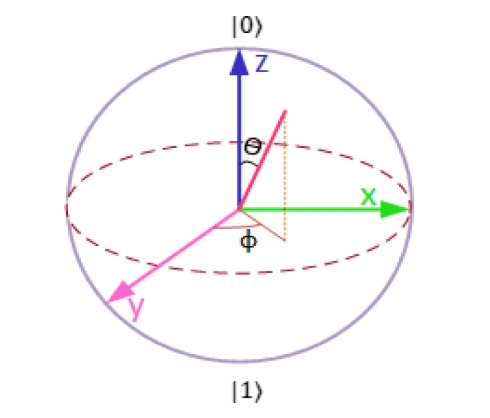
\includegraphics[width=.5\textwidth]{bloch.jpeg}}
\caption{بازنمایی کیوبیت در کره بلاچ}
\end{figure}
این بازنمایی را میتوانید به تعداد نامحدودی کیوبیت هم انطباق دهید. به طوری که با داشتن $n$ کیوبیت نیاز به نگهداری $n^{2}$ عدد خواهید داشت. این حالت زمانی رخ میدهد که $n$ کیوبیت درهم‌تنیده
\LTRfootnote{entangled}
 شوند به طوری که باهم یک حالت را تشکیل دهند و نتوان آن ها را جدا کرد. 
\cite{fundamentalsandapplications}
همچنان جمع مجذور همه ی مقادیر باید برابر با یک شود. نمایش انتزاعی دو کیوبیت به شکل زیر خواهد بود:
\begin{equation}
\left|\Psi\right\rangle = \alpha_{0}\left|00\right\rangle +  \alpha_{1}\left|01\right\rangle +  \alpha_{2}\left|10\right\rangle +  \alpha_{3}\left|11\right\rangle = \begin{bmatrix}
 \alpha_{0}
\\
 \alpha_{1}
\\
 \alpha_{2}
\\
 \alpha_{3}
\end{bmatrix}
\end{equation}
نمایش دو کیوبیت در فرم ماتریسی و دیراک
\LTRfootnote{Dirac}
:
\begin{equation}
\left|00\right\rangle  = \begin{bmatrix}
 \alpha_{1}
\\
 \alpha_{0}
\\
 \alpha_{0}
\\
 \alpha_{0}
\end{bmatrix}
\text{;}
\left|01\right\rangle  = \begin{bmatrix}
 \alpha_{0}
\\
 \alpha_{1}
\\
 \alpha_{0}
\\
 \alpha_{0}
\end{bmatrix}
\text{;}
\left|10\right\rangle  = \begin{bmatrix}
 \alpha_{0}
\\
 \alpha_{0}
\\
 \alpha_{1}
\\
 \alpha_{0}
\end{bmatrix}
\text{;}
\left|11\right\rangle  = \begin{bmatrix}
 \alpha_{0}
\\
 \alpha_{0}
\\
 \alpha_{0}
\\
 \alpha_{1}
\end{bmatrix}
\end{equation}


\subsection{ضرب تانسوری}
ضرب تانسوری
\LTRfootnote{Tensor product}
، عملیاتی است که بین دو ماتریس میتوان انجام داد. این عملیات، یکی از بخش های اصلی محاسبات کوانتومی است. برای اینکه بتوان سیستم های چند-کیوبیتی
\LTRfootnote{multiple-qubit systems}
را به صورت ریاضی نمایش داد، از این عملیات استفاده میشود. به این صورت که اگر $M$ یک ماتریس $(p,q)$ باشد و  $N$ یک ماتریس $(x,y)$ باشد، ماتریس ضرب تانسوری آنها یک ماتریس $(px,qy)$ خواهد بود. 
\cite{fundamentalsandapplications}
این ضرب را میتوان با یک گیت کوانتومی
\LTRfootnote{quantum gate}
 اعمال کرد.
\begin{equation}
M =  \begin{bmatrix}
 a_{11} &  a_{12}
\\
 a_{21} & a_{22}
\end{bmatrix}
\text{;}
N =  \begin{bmatrix}
 b_{11} &  b_{12}
\\
 b_{21} &  b_{22}
\end{bmatrix}
\end{equation}

\begin{equation}
M \oplus  N =  \begin{bmatrix}
 a_{11}b_{11} &  a_{11}b_{12} &  a_{12}b_{11} &  a_{12}b_{12}
\\
 a_{11}b_{21} &  a_{11}b_{22} &  a_{12}b_{21} &  a_{12}b_{22}
\\
 a_{21}b_{11} &  a_{21}b_{12} &  a_{22}b_{11} &  a_{22}b_{12}
\\
 a_{21}b_{21} &  a_{21}b_{22} &  a_{22}b_{21} &  a_{22}b_{22}
\end{bmatrix}
\end{equation}
برای ضرب تانسوری دو کیوبیت خواهیم داشت:
\begin{equation}
\left|0\right\rangle  \oplus  \left|1\right\rangle  =
\begin{bmatrix}
1 \\ 0 
\end{bmatrix} 
\oplus 
\begin{bmatrix}
0 \\ 1 
\end{bmatrix} 
=
  \begin{bmatrix}
0
\\
1
\\
0
\\
0
\end{bmatrix} = \left|01\right\rangle
\end{equation}

	

%--------------------------------------------------------------------------appendix( مراجع و پیوست ها)
\chapterfont{\vspace*{-2em}\centering\LARGE}%

\appendix
\bibliographystyle{plain-fa}
\bibliography{references}
%\chapter*{‌پیوست}
\markboth{پیوست}{}
\addcontentsline{toc}{chapter}{پیوست}
موضوعات مرتبط با متن گزارش پایان نامه كه در يكی از گروه‌های زير قرار می‌گيرد، در بخش پيوست‌ها آورده شوند:
\begin{enumerate}
\item  اثبات های رياضی يا عمليات رياضی طولانی‌.‌
\item داده و اطلاعات نمونه (های) مورد مطالعه (\lr{Case Study}) چنانچه طولانی باشد‌.‌
\item نتايج كارهای ديگران چنانچه نياز به تفصيل باشد‌.‌
\item مجموعه تعاريف متغيرها و پارامترها، چنانچه طولانی بوده و در متن به انجام نرسيده باشد‌.‌
\end{enumerate}
% براي شماره‌گذاري روابط، جداول و اشكال موجود در پيوست‌ از ساختار متفاوتي نسبت به متن اصلي استفاده مي‌شود كه در زير به‌عنوان نمونه نمايش داده شده‌است. 
% \begin{equation}
%F=ma
%\end{equation}
\section*{کد میپل }
\begin{latin}
\begin{verbatim}

with(DifferentialGeometry):
with(Tensor):
DGsetup([x, y, z], M)
																	frame name: M
a := evalDG(D_x)
																	D_x
b := evalDG(-2 y z D_x+2 x D_y/z^3-D_z/z^2)


\end{verbatim}
\end{latin}
%--------------------------------------------------------------------------dictionary(واژه نامه ها)
%اگر مایل به داشتن صفحه واژه‌نامه نیستید، خط زیر را غیر فعال کنید.
\parindent=0pt
%%
\chapter*{واژه‌نامه‌ی فارسی به انگلیسی}
\pagestyle{style9}

\addcontentsline{toc}{chapter}{واژه‌نامه‌ی فارسی به انگلیسی}
%%%%%%
\begin{multicols*}{2}

{\bf آ}
\vspace*{3mm}


\farsiTOenglish{اسکالر}{Scalar}


\vspace*{3mm}
{\bf ب}
\vspace*{3mm}

\farsiTOenglish{بالابر}{Lift}


\vspace*{3mm}
{\bf پ}
%%\vspace*{3mm}

\farsiTOenglish{پایا}{Invariant}



\vspace*{3mm}
{\bf ت}
%%\vspace*{3mm}

\farsiTOenglish{ تناظر }{Correspondence}


\vspace*{3mm}
{\bf ث}
%%\vspace*{3mm}

\farsiTOenglish{ثابت‌ساز}{Stabilizer}

\vspace*{3mm}
{\bf ج}
%%\vspace*{3mm}

\farsiTOenglish{جایگشت}{Permutation}



\vspace*{3mm}
{\bf چ}
%%\vspace*{3mm}


\farsiTOenglish{چند جمله‌ای }{Polynomial}

\vspace*{3mm}
{\bf ح}
%%\vspace*{3mm}

\farsiTOenglish{حاصل‌ضرب دکارتی}{Cartesian product}


\vspace*{3mm}
{\bf خ}
%%\vspace*{3mm}

\farsiTOenglish{خودریختی}{Automorphism}

\vspace*{3mm}
{\bf د}
%%\vspace*{3mm}

\farsiTOenglish{درجه}{Degree}


\vspace*{3mm}
{\bf ر}
%%\vspace*{3mm}


\farsiTOenglish{ریزپردازنده}{microprocessor}


\vspace*{3mm}
{\bf ز}
%%\vspace*{3mm}


\farsiTOenglish{زیرمدول}{Submodule}


\vspace*{3mm}
{\bf س}
%%\vspace*{3mm}

\farsiTOenglish{سرشت}{Character}


\vspace*{3mm}
{\bf ص}
%%\vspace*{3mm}

\farsiTOenglish{صادقانه}{Faithful}

\vspace*{3mm}
{\bf ض}
%%\vspace*{3mm}

\farsiTOenglish{ضرب داخلی}{Inner product}

\vspace*{3mm}
{\bf ط}
%%\vspace*{3mm}


\farsiTOenglish{طوقه}{Loop}


\vspace*{3mm}
{\bf ظ}
%%\vspace*{3mm}


\farsiTOenglish{ظرفیت}{Valency}
 
\vspace*{3mm}
{\bf ع}
%%\vspace*{3mm}


\farsiTOenglish{عدم مجاورت}{Nonadjacency}



\vspace*{3mm}
{\bf ف}
%%\vspace*{3mm}

\farsiTOenglish{فضای برداری}{Vector space}



\vspace*{3mm}
{\bf ک}
%%\vspace*{3mm}

\farsiTOenglish{کاملاً تحویل‌پذیر}{Complete reducibility}


\vspace*{3mm}
{\bf گ}
%%\vspace*{3mm}


\farsiTOenglish{گراف}{Graph}



\vspace*{3mm}
{\bf م}
%%\vspace*{3mm}

\farsiTOenglish{ماتریس جایگشتی}{Permutation matrix }


\vspace*{3mm}
{\bf ن}
%%\vspace*{3mm}

\farsiTOenglish{ناهمبند}{Disconnected}


\vspace*{3mm}
{\bf و}
%%\vspace*{3mm}

\farsiTOenglish{وارون‌پذیر}{Invertible}


\vspace*{3mm}
{\bf ه}
%%\vspace*{3mm}

\farsiTOenglish{همبند}{Connected}



\vspace*{3mm}
{\bf ی}
%%\vspace*{3mm}

\farsiTOenglish{یال}{Edge}




\end{multicols*}
%%%%%%%
\chapter*{ واژه‌نامه‌ی انگلیسی به فارسی}
\pagestyle{style9}
\lhead{\thepage}\rhead{واژه‌نامه‌ی انگلیسی به فارسی}
\addcontentsline{toc}{chapter}{واژه‌نامه‌ی انگلیسی به فارسی}

\LTRmulticolcolumns
\begin{multicols}{2}
{\hfill\bf  \lr{A}}
%%\vspace*{1.5mm}

\englishTOfarsi{Automorphism}{خودریختی}

\vspace*{3mm}
{\hfill\bf   \lr{B}}
%%\vspace*{1.5mm}

\englishTOfarsi{Bijection}{دوسویی}

\vspace*{3mm}
{\hfill\bf   \lr{C}}
%%\vspace*{1.5mm}

\englishTOfarsi{Cycle group}{گروه دوری}

\vspace*{3mm}
{\hfill\bf   \lr{D}}
%%\vspace*{1.5mm}

\englishTOfarsi{Degree}{درجه}

\vspace*{3mm}
{\hfill\bf   \lr{E}}
%%\vspace*{1.5mm}

\englishTOfarsi{Edge}{یال}

\vspace*{3mm}
{\hfill\bf   \lr{F}}
%%\vspace*{1.5mm}

\englishTOfarsi{Function}{تابع}

\vspace*{3mm}
{\hfill\bf   \lr{G}}
%%\vspace*{1.5mm}

\englishTOfarsi{Group}{گروه}

\vspace*{3mm}
{\hfill\bf   \lr{H}}
%%\vspace*{1.5mm}

\englishTOfarsi{Homomorphism}{همریختی}

\vspace*{3mm}
{\hfill\bf   \lr{I}}
%%\vspace*{1.5mm}

\englishTOfarsi{Invariant}{پایا}

\vspace*{3mm}
{\hfill\bf   \lr{L}}
%%\vspace*{1.5mm}

\englishTOfarsi{Lift}{بالابر}

\vspace*{3mm}
{\hfill\bf   \lr{M}}
%%\vspace*{1.5mm}

\englishTOfarsi{Module}{مدول}

\vspace*{3mm}
{\hfill\bf   \lr{N}}
%%\vspace*{1.5mm}

\englishTOfarsi{Natural map}{نگاشت طبیعی}

\vspace*{3mm}
{\hfill\bf   \lr{O}}
%%\vspace*{1.5mm}

\englishTOfarsi{One to One}{یک به یک}

\vspace*{3mm}
{\hfill\bf   \lr{P}}
%%\vspace*{1.5mm}

\englishTOfarsi{Permutation group}{گروه جایگشتی}

\vspace*{3mm}
{\hfill\bf   \lr{Q}}
%%\vspace*{1.5mm}

\englishTOfarsi{Quotient graph}{گراف خارج‌قسمتی}

 \vspace*{3mm}
{\hfill\bf   \lr{R}}
%%\vspace*{1.5mm}

\englishTOfarsi{Reducible}{تحویل پذیر}

\vspace*{3mm}
{\hfill\bf   \lr{S}}
%%\vspace*{1.5mm}

\englishTOfarsi{Sequence}{دنباله}

 \vspace*{3mm}
{\hfill\bf   \lr{T}}
%%\vspace*{1.5mm}

\englishTOfarsi{Trivial character}{سرشت بدیهی}

\vspace*{3mm}
{\hfill\bf   \lr{U}}
%%\vspace*{1.5mm}

\englishTOfarsi{Unique}{منحصربفرد}

\vspace*{3mm}
{\hfill\bf   \lr{V}}
%%\vspace*{1.5mm}

\englishTOfarsi{Vector space}{فضای برداری}
\end{multicols}
%--------------------------------------------------------------------------index(نمایه)
%اگر مایل به داشتن صفحه نمایه نیستید، خط زیر را غیر فعال کنید.
%\pagestyle{style7}
%\printindex
%\pagestyle{style7}
%%کلمات کلیدی انگلیسی
\latinkeywords{Write a 3 to 5 KeyWords is essential. Example: AUT, M.Sc., Ph. D,..}
%چکیده انگلیسی

\en-abstract{
This page is accurate translation from Persian abstract into English.
}
%%%%%%%%%%%%%%%%%%%%% کدهای زیر را تغییر ندهید.

\newpage
\thispagestyle{empty}
\begin{latin}
\section*{\LARGE\centering Abstract}

\een-abstract

\vspace*{.5cm}
{\large\textbf{Key Words:}}\par
\vspace*{.5cm}
\elatinkeywords
\end{latin}
%% در این فایل، عنوان پایان‌نامه، مشخصات خود و چکیده پایان‌نامه را به انگلیسی، وارد کنید.
%%%%%%%%%%%%%%%%%%%%%%%%%%%%%%%%%%%%
\baselineskip=.6cm
\begin{latin}

\latinfaculty{Department of computer engineering}


\latintitle{An introdunction to 	quantum computing from computer engineering standpoint}


\firstlatinsupervisor{Dr. Hamed Farbeh }

%\secondlatinsupervisor{Second Supervisor}

%\firstlatinadvisor{Dr. }

%\secondlatinadvisor{Second Advisor}

\latinname{Helia}

\latinsurname{Akbari}

\latinthesisdate{June 2024}

\latinvtitle
\end{latin}

\end{document}